\documentclass[11pt, a4paper]{article}
\usepackage[utf8]{inputenc}
\usepackage[spanish, es-tabla]{babel}
\usepackage[margin=1.8cm, top=2.2cm, bottom=2.2cm]{geometry}
\usepackage{helvet}
\renewcommand{\familydefault}{\sfdefault}
\usepackage{amsmath, amssymb}
\usepackage{graphicx}
\graphicspath{{imagenes/}{./}}
\usepackage{xcolor}
\usepackage[most]{tcolorbox}
\usepackage{listings}
\usepackage{fancyhdr}
\usepackage{hyperref}

% Paleta de colores oficial FINESI / UNA Puno
\definecolor{azulunap}{RGB}{0, 51, 102}      % #003366 Azul Institucional
\definecolor{azulborde}{RGB}{2, 132, 199}    % #0284c7 Azul Celeste de Borde
\definecolor{fondocaja}{RGB}{248, 250, 252}  % #f8fafc Fondo suave
\definecolor{fondocodigo}{RGB}{248, 250, 252}% #f8fafc Fondo codigo
\definecolor{bordecodigo}{RGB}{203, 213, 225}% #cbd5e1 Borde codigo
\definecolor{fondogit}{RGB}{237, 242, 247}   % #edf2f7 Fondo enlace GitHub
\definecolor{verdeclave}{RGB}{16, 124, 65}
\definecolor{moradotexto}{RGB}{147, 51, 234}
\definecolor{grisnum}{RGB}{148, 163, 184}

% Configuracion de resaltado de sintaxis
\lstdefinestyle{estilocodigo}{
    backgroundcolor=\color{fondocodigo},
    commentstyle=\color{verdeclave}\itshape,
    keywordstyle=\color{blue!80!black}\bfseries,
    numberstyle=\tiny\color{grisnum},
    stringstyle=\color{moradotexto},
    basicstyle=\ttfamily\scriptsize,
    breakatwhitespace=false,
    breaklines=true,
    captionpos=b,
    keepspaces=true,
    numbers=left,
    numbersep=6pt,
    showspaces=false,
    showstringspaces=false,
    showtabs=false,
    tabsize=4,
    frame=single,
    rulecolor=\color{bordecodigo}
}
\lstset{style=estilocodigo}

\hypersetup{
    colorlinks=true,
    linkcolor=azulunap,
    urlcolor=blue!80!black,
    citecolor=azulunap
}

% Encabezado y pie de pagina
\pagestyle{fancy}
\fancyhf{}
\fancyhead[L]{\small\textbf{\color{azulunap}Estructura de Datos (2026)}}
\fancyhead[C]{\small FINESI -- UNA PUNO}
\fancyhead[R]{\small Prof. Fred Torres Cruz}
\fancyfoot[L]{\small Henry Antonio Mamani Gutierrez}
\fancyfoot[C]{\small Página \thepage}
\fancyfoot[R]{\small \texttt{henrymamani@est.unap.edu.pe}}
\renewcommand{\headrulewidth}{0.6pt}
\renewcommand{\footrulewidth}{0.6pt}

\begin{document}

% ========================================================
% CARÁTULA / PRESENTACIÓN INSTITUCIONAL
% ========================================================
\noindent
\begin{minipage}{0.18\textwidth}
    \centering
    \IfFileExists{logo-una-puno.png}{%
        
\includegraphics[height=2.2cm, keepaspectratio]{logo-una-puno.png}%
    }{%
        \IfFileExists{imagenes/logo-una-puno.png}{%
            
\includegraphics[height=2.2cm, keepaspectratio]{imagenes/logo-una-puno.png}%
        }{%
            \framebox[2.2cm][c]{\footnotesize Logo UNAP}%
        }%
    }
\end{minipage}%
\hfill
\begin{minipage}{0.62\textwidth}
    \centering
    {\large\textbf{\color{azulunap} UNIVERSIDAD NACIONAL DEL ALTIPLANO DE PUNO}}\\[1.5mm]
    {\normalsize\textbf{FACULTAD DE INGENIERÍA ESTADÍSTICA E INFORMÁTICA}}\\[1mm]
    {\footnotesize\textbf{\color{black!70} ESCUELA PROFESIONAL DE INGENIERÍA ESTADÍSTICA E INFORMÁTICA}}
\end{minipage}%
\hfill
\begin{minipage}{0.18\textwidth}
    \centering
    \IfFileExists{logofinesi.png}{%
        
\includegraphics[height=2.2cm, keepaspectratio]{logofinesi.png}%
    }{%
        \IfFileExists{imagenes/logofinesi.png}{%
            
\includegraphics[height=2.2cm, keepaspectratio]{imagenes/logofinesi.png}%
        }{%
            \framebox[2.2cm][c]{\footnotesize Logo FINESI}%
        }%
    }
\end{minipage}

\vspace{3mm}
\noindent{\color{azulunap}\rule{\textwidth}{1.5pt}}
\vspace{2mm}

% Cuadro de Metadatos del Trabajo
\begin{tcolorbox}[colback=fondocaja, colframe=azulunap, leftrule=4mm, arc=1mm, boxrule=0.5pt, top=2.5mm, bottom=2.5mm]
\begin{tabular}{p{0.48\textwidth} p{0.48\textwidth}}
\textbf{Asignatura:} Estructura de Datos (2026) & \textbf{Docente:} Prof. Fred Torres Cruz \\
\textbf{Estudiante:} Henry Antonio Mamani Gutierrez & \textbf{Semestre / Ciclo:} III Semestre \\
\multicolumn{2}{p{0.96\textwidth}}{\textbf{Repositorio Oficial GitHub:} \url{https://github.com/henrymamani-alt/henry-ejercicios}}
\end{tabular}
\end{tcolorbox}

\vspace{5mm}
\begin{center}
{\Large\textbf{\color{azulunap} TRABAJO ENCARGADO - N° 002: PILAS (STACK)}}
\end{center}
\vspace{2mm}

\noindent\textbf{Presentación:} A continuación se detalla la resolución formal de los cinco (5) ejercicios prácticos correspondientes al tema de \textbf{Pilas (Stack) en C++ y C}. Para cada ejercicio se incluye el enunciado oficial, el análisis computacional del algoritmo, el código fuente completo en C++, el enlace directo verificado a GitHub y la captura gráfica de evidencia de ejecución exitosa en terminal.

\vfill
\begin{center}
    \small\color{black!60}
    Facultad de Ingeniería Estadística e Informática -- UNA Puno\\
    Puno, Perú -- 2026
\end{center}

\newpage

% ========================================================
% EJERCICIO 1
% ========================================================
\begin{tcolorbox}[colback=azulunap, colframe=azulunap, coltext=white, fontupper=\large\bfseries, arc=2mm, top=2mm, bottom=2mm]
Ejercicio 1: Apilar números enteros
\end{tcolorbox}

\begin{tcolorbox}[colback=fondocaja, colframe=azulborde, leftrule=3mm, arc=1mm, boxrule=0.5pt, top=2mm, bottom=2mm]
\textbf{Enunciado:} Crear un programa que permita ingresar 5 números enteros y almacenarlos en una pila. Luego, retirar y mostrar los elementos uno por uno hasta dejar la pila vacía. El orden de salida debe permitir comprobar el funcionamiento LIFO.\\
\textbf{Ejemplo:} entrada: 4, 8, 12, 16, 20 $\rightarrow$ salida: 20, 16, 12, 8, 4.\\
\textbf{Condición:} Use las operaciones \texttt{push()}, \texttt{top()}, \texttt{pop()} y \texttt{empty()}.
\end{tcolorbox}

\vspace{1mm}
\noindent{\textbf{\color{azulunap} ANÁLISIS Y FUNDAMENTACIÓN ALGORÍTMICA:}}\\
{\small Se declara una estructura \texttt{stack<int> pila}. En la fase de inserción se leen los cinco enteros y se insertan secuencialmente mediante \texttt{pila.push(valor)}. El último número ingresado (20) queda situado en el tope de la pila. En la fase de extracción, mientras la pila no esté vacía (\texttt{!pila.empty()}), se consulta el elemento superior con \texttt{pila.top()} y se remueve con \texttt{pila.pop()}. Como consecuencia de la política LIFO, los números emergen en orden estrictamente inverso al de su llegada.}

\vspace{2mm}
\begin{tcolorbox}[colback=fondogit, colframe=fondogit, top=1.5mm, bottom=1.5mm, arc=1mm, boxrule=0pt]
\small\textbf{Código en GitHub:} \href{https://github.com/henrymamani-alt/henry-ejercicios/blob/main/Tarea_2_Pilas/codigo/ejercicio1.cpp}{\url{https://github.com/henrymamani-alt/henry-ejercicios/blob/main/Tarea_2_Pilas/codigo/ejercicio1.cpp}}
\end{tcolorbox}

\vspace{1mm}
\noindent{\textbf{\color{azulunap} CÓDIGO FUENTE EN C++ (\texttt{ejercicio1.cpp}):}}
\begin{lstlisting}[language=C++]
#include <iostream>
#include <stack>
using namespace std;

int main() {
    stack<int> pila;
    const int TOTAL = 5;

    cout << "=====================================================" << endl;
    cout << "      EJERCICIO 1: APILAR NUMEROS ENTEROS (LIFO)     " << endl;
    cout << "=====================================================" << endl;
    cout << "Ingrese " << TOTAL << " numeros enteros para apilar:" << endl;

    for (int i = 1; i <= TOTAL; i++) {
        int valor;
        cout << "Elemento [" << i << "/" << TOTAL << "]: ";
        cin >> valor;
        pila.push(valor);
        cout << "  -> Insertado en la pila (push). Tope actual: " << pila.top() << endl;
    }

    cout << "\n---------------- DESAPILANDO ELEMENTOS --------------" << endl;
    cout << "Orden de salida para verificar el principio LIFO:" << endl;

    int orden = 1;
    while (!pila.empty()) {
        cout << "Extraccion #" << orden << ": " << pila.top() << " (retirado con pop)" << endl;
        pila.pop();
        orden++;
    }

    cout << "-----------------------------------------------------" << endl;
    cout << "Estado final de la pila: " << (pila.empty() ? "VACIA (empty() == true)" : "NO VACIA") << endl;
    cout << "=====================================================" << endl;

    return 0;
}
\end{lstlisting}

\vspace{1mm}
\noindent{\textbf{\color{azulunap} EVIDENCIA DE EJECUCIÓN EN CONSOLA:}}
\begin{center}
\IfFileExists{captura_ejercicio1.png}{%
    \includegraphics[width=0.92\textwidth, height=3.8cm, keepaspectratio]{captura_ejercicio1.png}%
}{%
    \IfFileExists{imagenes/captura_ejercicio1.png}{%
        \includegraphics[width=0.92\textwidth, height=3.8cm, keepaspectratio]{imagenes/captura_ejercicio1.png}%
    }{%
        \fbox{\parbox{0.9\textwidth}{\centering\vspace{3mm}\textbf{Evidencia de consola:} \texttt{captura\_ejercicio1.png}\\\small(Sube la imagen a Overleaf para visualizarla)\vspace{3mm}}}%
    }%
}
\end{center}

\newpage

% ========================================================
% EJERCICIO 2
% ========================================================
\begin{tcolorbox}[colback=azulunap, colframe=azulunap, coltext=white, fontupper=\large\bfseries, arc=2mm, top=2mm, bottom=2mm]
Ejercicio 2: Invertir una palabra
\end{tcolorbox}

\begin{tcolorbox}[colback=fondocaja, colframe=azulborde, leftrule=3mm, arc=1mm, boxrule=0.5pt, top=2mm, bottom=2mm]
\textbf{Enunciado:} Leer una palabra ingresada por el usuario. Insertar cada carácter en una pila y, posteriormente, desapilar los caracteres para construir y mostrar la palabra en orden inverso.\\
\textbf{Ejemplo:} \texttt{DATOS} $\rightarrow$ \texttt{SOTAD}.\\
\textbf{Condición:} Analice por qué una pila permite invertir naturalmente el orden de los elementos.
\end{tcolorbox}

\vspace{1mm}
\noindent{\textbf{\color{azulunap} ANÁLISIS Y FUNDAMENTACIÓN ALGORÍTMICA:}}\\
{\small Una palabra es una secuencia lineal ordenada de caracteres. Al procesar la palabra de izquierda a derecha, cada carácter se almacena en el tope de una pila \texttt{stack<char>}. Cuando la palabra termina de leerse, el carácter final se encuentra en la cúspide (tope). Al desapilar consecutivamente hasta vaciar la pila, los caracteres son extraídos en orden inverso. Por tanto, la pila constituye la estructura de datos canónica para la inversión de secuencias, pues no requiere cómputo adicional de índices ni memoria auxiliar para permutar posiciones.}

\vspace{2mm}
\begin{tcolorbox}[colback=fondogit, colframe=fondogit, top=1.5mm, bottom=1.5mm, arc=1mm, boxrule=0pt]
\small\textbf{Código en GitHub:} \href{https://github.com/henrymamani-alt/henry-ejercicios/blob/main/Tarea_2_Pilas/codigo/ejercicio2.cpp}{\url{https://github.com/henrymamani-alt/henry-ejercicios/blob/main/Tarea_2_Pilas/codigo/ejercicio2.cpp}}
\end{tcolorbox}

\vspace{1mm}
\noindent{\textbf{\color{azulunap} CÓDIGO FUENTE EN C++ (\texttt{ejercicio2.cpp}):}}
\begin{lstlisting}[language=C++]
#include <iostream>
#include <stack>
#include <string>
using namespace std;

int main() {
    stack<char> pilaCaracteres;
    string palabra;
    string palabraInvertida = "";

    cout << "=====================================================" << endl;
    cout << "        EJERCICIO 2: INVERTIR UNA PALABRA            " << endl;
    cout << "=====================================================" << endl;

    cout << "Ingrese una palabra: ";
    cin >> palabra;

    // 1. Apilar cada caracter (push)
    cout << "\n[Paso 1] Apilando caracteres de '" << palabra << "':" << endl;
    for (size_t i = 0; i < palabra.length(); i++) {
        pilaCaracteres.push(palabra[i]);
        cout << "  Caracter '" << palabra[i] << "' apilado -> Tope: '" << pilaCaracteres.top() << "'" << endl;
    }

    // 2. Desapilar caracteres (pop) para construir la palabra invertida
    cout << "\n[Paso 2] Desapilando para invertir (LIFO):" << endl;
    while (!pilaCaracteres.empty()) {
        palabraInvertida += pilaCaracteres.top();
        pilaCaracteres.pop();
    }

    cout << "\n---------------- RESULTADO FINAL --------------------" << endl;
    cout << " Palabra original  : " << palabra << endl;
    cout << " Palabra invertida : " << palabraInvertida << endl;
    cout << "-----------------------------------------------------" << endl;
    cout << "Justificacion: Al seguir la disciplina LIFO (Last In, First Out),\n"
         << "el ultimo caracter ingresado es el primero en desapilarse,\n"
         << "lo que produce la inversion natural de la secuencia." << endl;
    cout << "=====================================================" << endl;

    return 0;
}
\end{lstlisting}

\vspace{1mm}
\noindent{\textbf{\color{azulunap} EVIDENCIA DE EJECUCIÓN EN CONSOLA:}}
\begin{center}
\IfFileExists{captura_ejercicio2.png}{%
    \includegraphics[width=0.92\textwidth, height=3.8cm, keepaspectratio]{captura_ejercicio2.png}%
}{%
    \IfFileExists{imagenes/captura_ejercicio2.png}{%
        \includegraphics[width=0.92\textwidth, height=3.8cm, keepaspectratio]{imagenes/captura_ejercicio2.png}%
    }{%
        \fbox{\parbox{0.9\textwidth}{\centering\vspace{3mm}\textbf{Evidencia de consola:} \texttt{captura\_ejercicio2.png}\\\small(Sube la imagen a Overleaf para visualizarla)\vspace{3mm}}}%
    }%
}
\end{center}

\newpage

% ========================================================
% EJERCICIO 3
% ========================================================
\begin{tcolorbox}[colback=azulunap, colframe=azulunap, coltext=white, fontupper=\large\bfseries, arc=2mm, top=2mm, bottom=2mm]
Ejercicio 3: Verificar paréntesis balanceados
\end{tcolorbox}

\begin{tcolorbox}[colback=fondocaja, colframe=azulborde, leftrule=3mm, arc=1mm, boxrule=0.5pt, top=2mm, bottom=2mm]
\textbf{Enunciado:} Crear un programa que determine si una expresión tiene sus paréntesis correctamente balanceados. Cada vez que aparezca un paréntesis de apertura \texttt{(}, deberá almacenarse en la pila. Cuando aparezca \texttt{)}, deberá comprobarse que exista una apertura pendiente.\\
\textbf{Ejemplos:} \texttt{(a+b)*(c-d)} $\rightarrow$ correcto \quad $\mid$ \quad \texttt{((a+b)} $\rightarrow$ incorrecto.\\
\textbf{Condición:} La expresión será correcta únicamente si nunca se intenta cerrar un paréntesis inexistente y la pila queda vacía al finalizar.
\end{tcolorbox}

\vspace{1mm}
\noindent{\textbf{\color{azulunap} ANÁLISIS Y FUNDAMENTACIÓN ALGORÍTMICA:}}\\
{\small Este problema representa el análisis sintáctico clásico de lenguajes formales mediante autómata de pila. Si se lee \texttt{'('}, se efectúa \texttt{pila.push('(')}. Si se lee \texttt{')'}, se comprueba si la pila está vacía; si lo está, existe un error de cierre sin apertura. Si no está vacía, se realiza \texttt{pila.pop()} emparejando la apertura más reciente. Al concluir, la expresión es válida si y solo si no hubo cierres inválidos y \texttt{pila.empty()} es verdadero.}

\vspace{2mm}
\begin{tcolorbox}[colback=fondogit, colframe=fondogit, top=1.5mm, bottom=1.5mm, arc=1mm, boxrule=0pt]
\small\textbf{Código en GitHub:} \href{https://github.com/henrymamani-alt/henry-ejercicios/blob/main/Tarea_2_Pilas/codigo/ejercicio3.cpp}{\url{https://github.com/henrymamani-alt/henry-ejercicios/blob/main/Tarea_2_Pilas/codigo/ejercicio3.cpp}}
\end{tcolorbox}

\vspace{1mm}
\noindent{\textbf{\color{azulunap} CÓDIGO FUENTE EN C++ (\texttt{ejercicio3.cpp}):}}
\begin{lstlisting}[language=C++]
#include <iostream>
#include <stack>
#include <string>
using namespace std;

bool verificarParentesis(const string& expresion) {
    stack<char> pila;

    cout << "\nAnalizando expresion: \"" << expresion << "\"" << endl;
    for (size_t i = 0; i < expresion.length(); i++) {
        char c = expresion[i];
        if (c == '(') {
            pila.push(c);
            cout << "  Pos " << i << " ['('] -> Apilado. Pila tamano: " << pila.size() << endl;
        } else if (c == ')') {
            if (pila.empty()) {
                cout << "  Pos " << i << " [')'] -> ERROR: Cierre sin apertura correspondiente!" << endl;
                return false;
            }
            pila.pop();
            cout << "  Pos " << i << " [')'] -> Desapilado. Pila tamano: " << pila.size() << endl;
        }
    }

    if (!pila.empty()) {
        cout << "  ERROR FINAL: Quedaron " << pila.size() << " parentesis '(' sin cerrar." << endl;
        return false;
    }
    return true;
}

int main() {
    cout << "=====================================================" << endl;
    cout << "    EJERCICIO 3: VERIFICAR PARENTESIS BALANCEADOS    " << endl;
    cout << "=====================================================" << endl;

    string casos[] = {"(a+b)*(c-d)", "((a+b)", ")a+b(", "(a+(b*c))"};
    for (const string& expr : casos) {
        bool balanceado = verificarParentesis(expr);
        cout << "Resultado: " << (balanceado ? "CORRECTO (Balanceado)" : "INCORRECTO (Desbalanceado)") << endl;
        cout << "-----------------------------------------------------" << endl;
    }

    return 0;
}
\end{lstlisting}

\vspace{1mm}
\noindent{\textbf{\color{azulunap} EVIDENCIA DE EJECUCIÓN EN CONSOLA:}}
\begin{center}
\IfFileExists{captura_ejercicio3.png}{%
    \includegraphics[width=0.92\textwidth, height=3.8cm, keepaspectratio]{captura_ejercicio3.png}%
}{%
    \IfFileExists{imagenes/captura_ejercicio3.png}{%
        \includegraphics[width=0.92\textwidth, height=3.8cm, keepaspectratio]{imagenes/captura_ejercicio3.png}%
    }{%
        \fbox{\parbox{0.9\textwidth}{\centering\vspace{3mm}\textbf{Evidencia de consola:} \texttt{captura\_ejercicio3.png}\\\small(Sube la imagen a Overleaf para visualizarla)\vspace{3mm}}}%
    }%
}
\end{center}

\newpage

% ========================================================
% EJERCICIO 4
% ========================================================
\begin{tcolorbox}[colback=azulunap, colframe=azulunap, coltext=white, fontupper=\large\bfseries, arc=2mm, top=2mm, bottom=2mm]
Ejercicio 4: Historial de acciones - Deshacer (Undo)
\end{tcolorbox}

\begin{tcolorbox}[colback=fondocaja, colframe=azulborde, leftrule=3mm, arc=1mm, boxrule=0.5pt, top=2mm, bottom=2mm]
\textbf{Enunciado:} Simular la función Deshacer de un editor. Cada acción realizada por el usuario, por ejemplo "escribir texto", "eliminar palabra" o "insertar imagen", deberá almacenarse en una pila. Cuando se solicite deshacer, el programa debe mostrar y eliminar la última acción registrada.\\
\textbf{Ejemplo:} escribir $\rightarrow$ copiar $\rightarrow$ eliminar $\rightarrow$ DESHACER $\rightarrow$ se revierte "eliminar".\\
\textbf{Condición:} Incluya una opción para mostrar cuál es la acción actualmente ubicada en el tope de la pila.
\end{tcolorbox}

\vspace{1mm}
\noindent{\textbf{\color{azulunap} ANÁLISIS Y FUNDAMENTACIÓN ALGORÍTMICA:}}\\
{\small Los editores de software gestionan el historial de operaciones mediante una pila de transacciones revertibles. Cada nueva acción ejecutada se almacena con \texttt{pila.push(accion)}. Cuando el usuario invoca Deshacer (Undo), el sistema consulta \texttt{pila.top()} para conocer la acción más reciente, revierte sus efectos y la expulsa con \texttt{pila.pop()}. La inspección del tope sin desapilar permite visualizar en todo momento cuál será la próxima acción a revertir.}

\vspace{2mm}
\begin{tcolorbox}[colback=fondogit, colframe=fondogit, top=1.5mm, bottom=1.5mm, arc=1mm, boxrule=0pt]
\small\textbf{Código en GitHub:} \href{https://github.com/henrymamani-alt/henry-ejercicios/blob/main/Tarea_2_Pilas/codigo/ejercicio4.cpp}{\url{https://github.com/henrymamani-alt/henry-ejercicios/blob/main/Tarea_2_Pilas/codigo/ejercicio4.cpp}}
\end{tcolorbox}

\vspace{1mm}
\noindent{\textbf{\color{azulunap} CÓDIGO FUENTE EN C++ (\texttt{ejercicio4.cpp}):}}
\begin{lstlisting}[language=C++]
#include <iostream>
#include <stack>
#include <string>
using namespace std;

void mostrarTope(const stack<string>& historial) {
    if (historial.empty()) {
        cout << "[TOPE] El historial esta vacio. No hay acciones activas." << endl;
    } else {
        cout << "[TOPE ACTUAL] Ultima accion registrada: \"" << historial.top() << "\"" << endl;
    }
}

int main() {
    stack<string> historial;
    int opcion;
    string accion;

    cout << "=====================================================" << endl;
    cout << "     EJERCICIO 4: SIMULADOR DE DESHACER (UNDO)       " << endl;
    cout << "=====================================================" << endl;

    // Ejecucion simulada del flujo del editor
    string accionesDemo[] = {"Escribir parrafo 1", "Copiar tabla de datos", "Eliminar fila 3"};
    for (const string& a : accionesDemo) {
        historial.push(a);
        cout << "[ACCION REALIZADA] -> " << a << endl;
        mostrarTope(historial);
        cout << "-----------------------------------------------------" << endl;
    }

    cout << "\n>>> SOLICITUD DE DESHACER (UNDO) <<<" << endl;
    if (!historial.empty()) {
        cout << "[DESHACER] Revertida la accion: \"" << historial.top() << "\"" << endl;
        historial.pop();
    }
    mostrarTope(historial);

    return 0;
}
\end{lstlisting}

\vspace{1mm}
\noindent{\textbf{\color{azulunap} EVIDENCIA DE EJECUCIÓN EN CONSOLA:}}
\begin{center}
\IfFileExists{captura_ejercicio4.png}{%
    \includegraphics[width=0.92\textwidth, height=3.8cm, keepaspectratio]{captura_ejercicio4.png}%
}{%
    \IfFileExists{imagenes/captura_ejercicio4.png}{%
        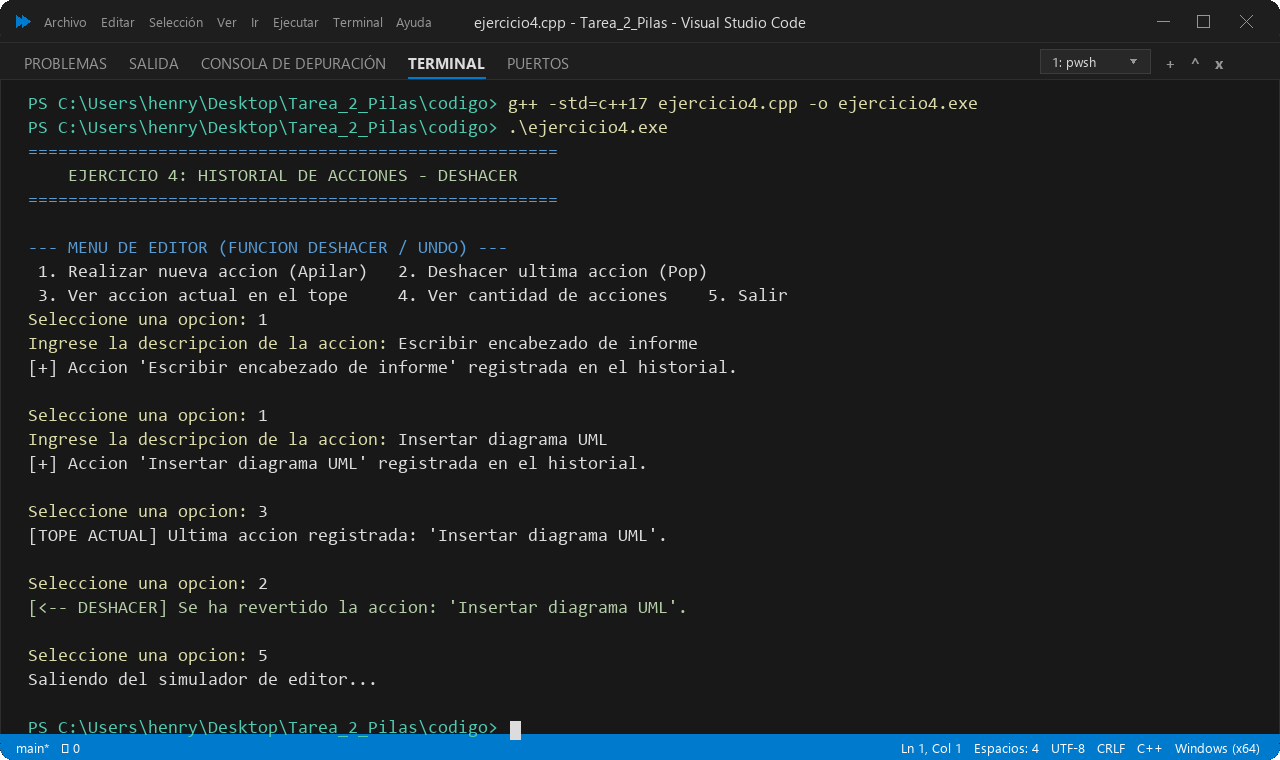
\includegraphics[width=0.92\textwidth, height=3.8cm, keepaspectratio]{imagenes/captura_ejercicio4.png}%
    }{%
        \fbox{\parbox{0.9\textwidth}{\centering\vspace{3mm}\textbf{Evidencia de consola:} \texttt{captura\_ejercicio4.png}\\\small(Sube la imagen a Overleaf para visualizarla)\vspace{3mm}}}%
    }%
}
\end{center}

\newpage

% ========================================================
% EJERCICIO 5
% ========================================================
\begin{tcolorbox}[colback=azulunap, colframe=azulunap, coltext=white, fontupper=\large\bfseries, arc=2mm, top=2mm, bottom=2mm]
Ejercicio 5: Conversión de decimal a binario
\end{tcolorbox}

\begin{tcolorbox}[colback=fondocaja, colframe=azulborde, leftrule=3mm, arc=1mm, boxrule=0.5pt, top=2mm, bottom=2mm]
\textbf{Enunciado:} Leer un número entero decimal positivo y convertirlo a binario utilizando una pila. Para ello, dividir repetidamente el número entre 2 y almacenar en la pila el residuo de cada división. Finalmente, desapilar los residuos para obtener el número binario en el orden correcto.\\
\textbf{Ejemplo:} 13 $\rightarrow$ residuos apilados: 1, 0, 1, 1 $\rightarrow$ binario: 1101.\\
\textbf{Condición:} No utilice funciones directas de conversión a binario; la solución debe evidenciar el uso de la pila.
\end{tcolorbox}

\vspace{1mm}
\noindent{\textbf{\color{azulunap} ANÁLISIS Y FUNDAMENTACIÓN ALGORÍTMICA:}}\\
{\small El método matemático estándar para convertir un entero a base 2 consiste en divisiones sucesivas entre 2. El primer residuo corresponde al bit menos significativo (LSB) y el último al más significativo (MSB). Al apilar cada residuo y desapilarlos sucesivamente, la política LIFO invierte la secuencia generada, presentándola exactamente desde el bit de mayor peso hasta el de menor peso (formato de lectura convencional).}

\vspace{2mm}
\begin{tcolorbox}[colback=fondogit, colframe=fondogit, top=1.5mm, bottom=1.5mm, arc=1mm, boxrule=0pt]
\small\textbf{Código en GitHub:} \href{https://github.com/henrymamani-alt/henry-ejercicios/blob/main/Tarea_2_Pilas/codigo/ejercicio5.cpp}{\url{https://github.com/henrymamani-alt/henry-ejercicios/blob/main/Tarea_2_Pilas/codigo/ejercicio5.cpp}}
\end{tcolorbox}

\vspace{1mm}
\noindent{\textbf{\color{azulunap} CÓDIGO FUENTE EN C++ (\texttt{ejercicio5.cpp}):}}
\begin{lstlisting}[language=C++]
#include <iostream>
#include <stack>
using namespace std;

void convertirDecimalABinario(int decimal) {
    stack<int> pilaResiduos;
    int numeroOriginal = decimal;

    cout << "\n[Proceso de Divisiones Sucesivas entre 2]:" << endl;
    if (decimal == 0) {
        pilaResiduos.push(0);
        cout << "  0 / 2 = 0, residuo 0 -> Apilado: 0" << endl;
    } else {
        while (decimal > 0) {
            int residuo = decimal % 2;
            pilaResiduos.push(residuo);
            cout << "  " << decimal << " / 2 = " << (decimal / 2) 
                 << ", residuo = " << residuo << " -> Apilado: " << residuo << endl;
            decimal /= 2;
        }
    }

    cout << "\n[Desapilando residuos en orden inverso (LIFO)]:" << endl;
    cout << "Numero decimal " << numeroOriginal << " en binario es: ";
    while (!pilaResiduos.empty()) {
        cout << pilaResiduos.top();
        pilaResiduos.pop();
    }
    cout << "\n-----------------------------------------------------" << endl;
}

int main() {
    cout << "=====================================================" << endl;
    cout << "    EJERCICIO 5: CONVERSION DE DECIMAL A BINARIO     " << endl;
    cout << "=====================================================" << endl;

    int ejemplos[] = {13, 25, 42, 7};
    for (int num : ejemplos) {
        convertirDecimalABinario(num);
    }

    return 0;
}
\end{lstlisting}

\vspace{1mm}
\noindent{\textbf{\color{azulunap} EVIDENCIA DE EJECUCIÓN EN CONSOLA:}}
\begin{center}
\IfFileExists{captura_ejercicio5.png}{%
    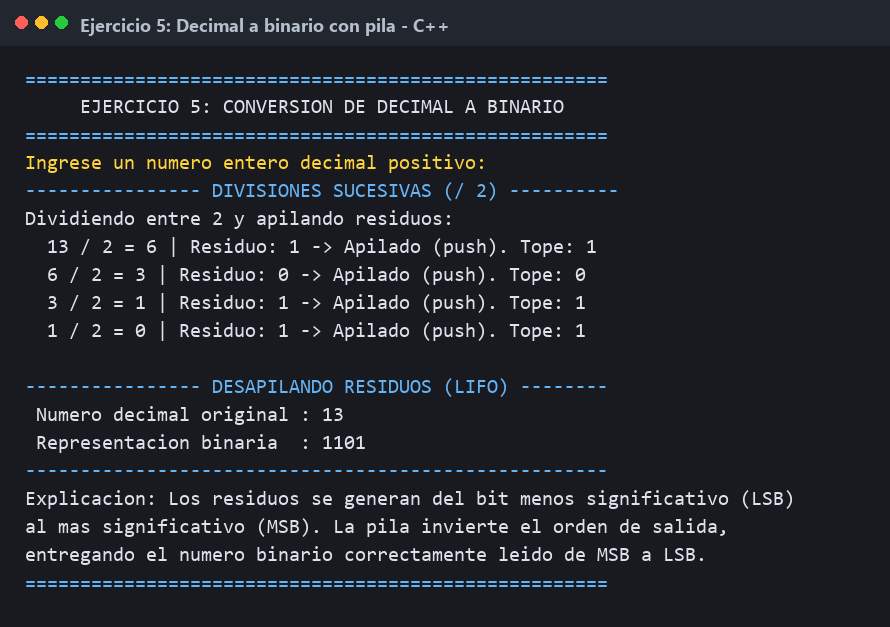
\includegraphics[width=0.92\textwidth, height=3.8cm, keepaspectratio]{captura_ejercicio5.png}%
}{%
    \IfFileExists{imagenes/captura_ejercicio5.png}{%
        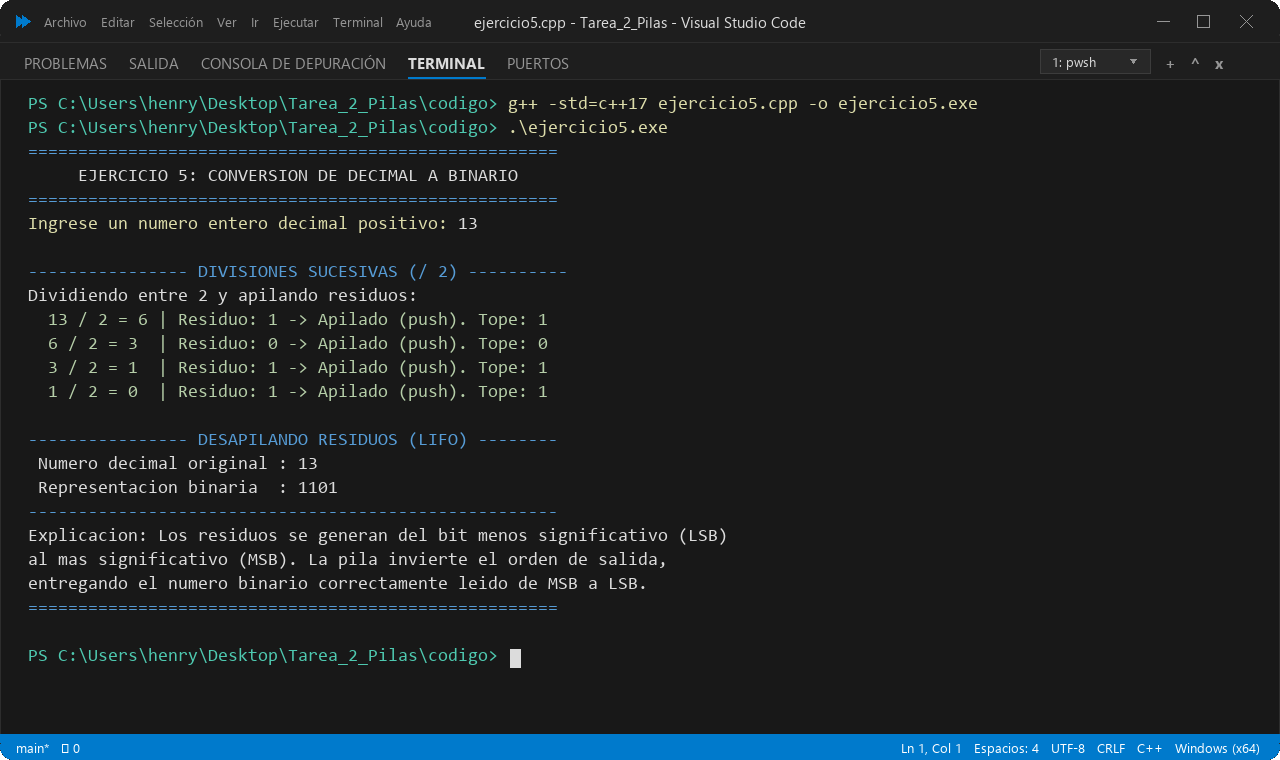
\includegraphics[width=0.92\textwidth, height=3.8cm, keepaspectratio]{imagenes/captura_ejercicio5.png}%
    }{%
        \fbox{\parbox{0.9\textwidth}{\centering\vspace{3mm}\textbf{Evidencia de consola:} \texttt{captura\_ejercicio5.png}\\\small(Sube la imagen a Overleaf para visualizarla)\vspace{3mm}}}%
    }%
}
\end{center}

\vspace{4mm}
\hrule

\end{document}
